\documentclass{article}

\PassOptionsToPackage{numbers, compress}{natbib}
\usepackage[final]{neurips_2019}

\usepackage[utf8]{inputenc}
\usepackage[T1]{fontenc}
\usepackage{hyperref}
\usepackage{url}
\usepackage{booktabs}
\usepackage{amsmath}
\usepackage{amssymb}
\usepackage{amsfonts}
\usepackage{microtype}
\usepackage{graphicx}
\usepackage{xcolor}

\hypersetup{
  colorlinks=true,
  linkcolor=blue!60!black,
  citecolor=blue!60!black,
  urlcolor=blue!60!black
}

\setlength{\textfloatsep}{7pt plus 2pt minus 2pt}
\setlength{\floatsep}{5pt plus 2pt minus 2pt}
\setlength{\intextsep}{5pt plus 2pt minus 2pt}

\title{Auditing Shortcut Learning and Chemical Out-of-Distribution Generalization in Multimodal Glioblastoma Drug Response Prediction}

\author{%
  Pan Chenan \quad (Student ID: G2604996F)\thanks{Course Final Mini-Project for \emph{MD6329: Deep Learning in Healthcare AI}, Nanyang Technological University (NTU). Project Showcase \& Interactive LecTrace Demo: \url{https://mnemopolis.github.io/gbm_drug_response_project/}. Source Code \& Reproducible Pipeline: \url{https://github.com/mnemopolis/gbm_drug_response_project}.} \\
  M.Sc.\ in AI in Medicine, Lee Kong Chian School of Medicine \\
  Nanyang Technological University, Singapore \\
  \texttt{PANC0010@e.ntu.edu.sg}
}

\begin{document}

\maketitle

\begin{abstract}
Predicting anticancer drug sensitivity ($\text{LN\_IC50}$) from tumor multi-omics profiles and molecular structures is a core task in computational oncology. On standard in-distribution random splits, multimodal deep learning models frequently report Spearman rank correlations above $0.85$. In this work, we investigate whether high correlation on random splits reflects learned drug--gene interactions or a statistical shortcut driven by between-drug potency differences. We construct a leakage-free benchmark for Glioblastoma (GBM) combining GDSC2 dose-response assays, DepMap transcriptomics, somatic hotspot mutations, promoter methylation, and RDKit molecular fingerprints across $5,107$ unique $(\text{drug}, \text{cell line})$ pairs ($24$ GBM cell lines and $243$ drugs). We evaluate a Two-Tower Multi-Layer Perceptron (\texttt{BaselineMLP}) implementing Joint (Intermediate) Fusion against closed-form statistical baselines across three evaluation regimes: Random (in-distribution), Leave-Cell-Out (unseen patient cell lines), and Bemis--Murcko Scaffold (unseen chemical structures) across $5$ random seeds. First, on the Random split, an interaction-free additive baseline ($\bar{y}_d + \bar{y}_c - \bar{y}_{\text{global}}$) achieves a Spearman correlation of $0.8752$, matching \texttt{BaselineMLP} ($0.8744 \pm 0.0051$) and showing that $95.5\%$ of the explainable rank correlation comes from memorizing average drug toxicity (\texttt{Drug-Only} $r_s = 0.8349$). Second, when evaluating on unseen chemical scaffolds, where drug-identity lookup is impossible, global Spearman drops to $0.2905 \pm 0.0045$ and RMSE increases from $1.0346$ to $2.1951$ due to severe prediction variance shrinkage toward the training mean ($\sigma(\hat{y})/\sigma(y) = 0.663$). Third, despite global collapse on unseen scaffolds, the median within-drug Spearman correlation across the $24$ GBM cell lines remains $0.530$ (compared to $0.500$ on Random and Leave-Cell-Out). This decoupling shows that the multi-omics cell encoder preserves relative patient susceptibility ranking for novel compounds, whereas the primary bottleneck in chemical out-of-distribution generalization is calibrating the per-drug baseline potency offset.
\end{abstract}

\section{Problem formulation}
\label{sec:problem}

\subsection{Clinical motivation in Glioblastoma}
Glioblastoma (GBM, World Health Organization Grade IV astrocytoma) is the most common and aggressive primary malignant brain tumor in adults. Under the standard Stupp protocol---maximal safe surgical resection followed by concomitant radiotherapy and oral chemotherapy with the DNA-alkylating agent Temozolomide (TMZ)---median overall survival remains under $15$ months, and five-year survival is below $7\%$~\cite{stupp2005radiotherapy}. Clinical response to TMZ and salvage therapies (such as Lomustine, Carmustine, Irinotecan, and Etoposide) varies widely across patients due to intratumoral and interpatient molecular heterogeneity~\cite{brennan2013somatic}. A key clinical biomarker in GBM is epigenetic silencing of the $O^6$-methylguanine-DNA methyltransferase (\texttt{MGMT}) gene via promoter methylation: tumors with low \texttt{MGMT} expression cannot efficiently repair $O^6$-methylguanine DNA lesions induced by TMZ and are more sensitive to alkylating chemotherapy, whereas \texttt{MGMT}-high tumors exhibit resistance~\cite{hegi2005mgmt}. Together with recurrent somatic alterations in \texttt{PTEN}, \texttt{TP53}, \texttt{EGFR}, and \texttt{RB1}, these molecular features motivate computational models that predict drug sensitivity from multi-omics profiles.

\subsection{The random-split evaluation pitfall and research questions}
Preclinical drug response models are typically trained on high-throughput cell-line screening panels such as the Genomics of Drug Sensitivity in Cancer (GDSC2)~\cite{yang2013gdsc,iorio2016landscape}, where sensitivity is quantified by the natural logarithm of the half-maximal inhibitory concentration ($\text{LN\_IC50}$, in $\ln\,\mu\text{M}$). Most published deep learning studies evaluate models using an in-distribution \emph{random pair split}, holding out $20\%$ of $(\text{drug}, \text{cell line})$ pairs at random. Under this setup, the same $243$ drugs and $24$ GBM cell lines appear in both the training and test sets. Because screened compounds span a wide range of intrinsic potencies---from general cytotoxic agents such as Docetaxel ($\text{mean LN\_IC50} = -4.12$) to weak in-vitro alkylators such as Temozolomide ($\text{mean LN\_IC50} = +6.45$)---between-drug variance is much larger than between-cell-line variance within a given drug~\cite{li2021audit}. Consequently, a neural network can achieve a high pooled correlation on a random split simply by memorizing each drug's mean $\text{LN\_IC50}$, without learning how specific transcriptomic or mutational profiles modulate drug response.

To test whether a multimodal neural network learns biological drug--cell interactions or relies on drug-mean memorization, we formulate three research questions:
\begin{itemize}
  \setlength{\itemsep}{1pt}\setlength{\parskip}{0pt}\setlength{\topsep}{2pt}
  \item \textbf{RQ1 (Shortcut audit on in-distribution splits):} How much of the test Spearman rank correlation achieved by a Two-Tower multimodal neural network (\texttt{BaselineMLP}) on a random split exceeds a zero-interaction additive baseline ($\hat{y}_{d,c} = \bar{y}_d + \bar{y}_c - \bar{y}_{\text{global}}$) that sums marginal drug and cell-line training means?
  \item \textbf{RQ2 (Biological vs.\ chemical out-of-distribution shift):} How does predictive performance degrade when generalizing to unseen GBM patient cell lines (\emph{Leave-Cell-Out split}) versus unseen Bemis--Murcko chemical scaffolds (\emph{Scaffold split}), and how does prediction variance shrinkage ($\sigma(\hat{y})/\sigma(y)$) behave across these regimes?
  \item \textbf{RQ3 (Decoupling between global and within-drug ranking):} When global pooled correlation drops on unseen chemical scaffolds, does the model lose all predictive signal, or does the multi-omics cell encoder still rank relative cell-line susceptibility \emph{within} each novel drug?
\end{itemize}

\paragraph{Hypothesis and study plan.}
We hypothesize that (i) random-split performance in GBM drug response prediction is dominated by drug-level main effects with negligible nonlinear interaction gain over an additive baseline, (ii) Leave-Cell-Out performance remains high because known drug mean potencies transfer across GBM cell lines, and (iii) Scaffold splitting removes the drug-identity shortcut, causing predictions to shrink toward the global training mean and degrading global correlation while preserving within-drug relative patient rankings.

\subsection{Role of Software 3.0 (Generative AI copilots) in problem formulation}
During initial scoping, we used DeepSeek for early project ideation, problem conceptualization, and modular system architecture design, alongside Gemini for baseline prototyping and code implementation. Initial AI suggestions proposed replacing fingerprint encoders with deeper graph attention networks and cross-modal transformers to push random-split Spearman correlation from $0.87$ toward $0.91$. When we inspected the empirical $\text{LN\_IC50}$ distributions, however, we observed that drug-level means spanned over $10$ log units whereas cell-line means varied by less than $1.5$ log units. We prompted the AI copilots to help implement closed-form marginal baselines (\texttt{Cell-Only}, \texttt{Drug-Only}, and \texttt{Additive}), which revealed that the zero-interaction additive baseline matched the neural network on the random split ($0.8752$ vs.\ $0.8744$). This check led us to reject the initial suggestion of chasing higher random-split accuracy with heavier architectures, and instead focus on out-of-distribution (OOD) auditing, variance shrinkage, and metric decoupling.

\section{Related work}
\label{sec:related}

\paragraph{Pharmacogenomic screens and multimodal drug response models.}
Large-scale pharmacogenomic repositories, including GDSC~\cite{yang2013gdsc,iorio2016landscape} and CCLE / DepMap~\cite{barretina2012ccle,tsherniak2017depmap,ghandi2019next}, have enabled data-driven modeling of cancer drug sensitivity. Early approaches used elastic net regression, random forests, or kernel methods over gene expression profiles~\cite{iorio2016landscape,costello2014community}. Subsequent deep learning models introduced two-tower intermediate/joint-fusion architectures~\cite{huang2020fusion} that separately encode drug structures and cellular multi-omics features before concatenating latent representations to predict $\text{IC}_{50}$. Representative models include CDRscan~\cite{chang2018cdrscan}, which applies convolutional layers to mutation profiles and molecular fingerprints; DeepCDR~\cite{liu2020deepcdr}, which combines a hybrid graph convolutional network with multi-omics subnetworks for transcriptomics, genomics, and epigenomics; GraphDRP~\cite{nguyen2021graphdrp}, which benchmarks GIN and GCN molecular graph encoders against 1D convolutional omics encoders; and TGSA~\cite{zhu2022tgsa}, which incorporates protein--protein interaction priors into cell-line graphs. While these studies report strong correlations ($r_s \in [0.85, 0.92]$) on random pair splits, most do not quantify how much of that correlation is already explained by marginal drug averages.

\paragraph{Molecular representations and chemical scaffold splitting.}
Extended-Connectivity Fingerprints (ECFPs / Morgan circular fingerprints)~\cite{rogers2010ecfp} in RDKit~\cite{landrum2016rdkit} hash circular atomic neighborhoods of radius $r$ into fixed-length bit vectors. For evaluating chemical generalization, Bemis and Murcko~\cite{bemis1996properties} decomposed drug molecules into ring systems, linkers, and side chains, and MoleculeNet~\cite{wu2018moleculenet} established Bemis--Murcko scaffold splitting as a standard benchmark for testing generalization to novel chemical series. On molecular graphs, Xu et al.~\cite{xu2019powerful} showed that Graph Isomorphism Networks (GIN) match the discriminative power of the Weisfeiler--Lehman isomorphism test, motivating our inclusion of both a Morgan fingerprint MLP tower and a GIN graph encoder (\texttt{GNNDrugMLP}).

\paragraph{Shortcut learning and cold-start auditing in biomedical AI.}
Geirhos et al.~\cite{geirhos2020shortcut} characterized \emph{shortcut learning} as the reliance of neural networks on simple marginal regularities that succeed on i.i.d.\ splits but fail under distribution shift. In pharmacogenomics, Li et al.~\cite{li2021audit} and Sharifi-Noghabi et al.~\cite{sharifi2021out} showed that pooling multiple drugs into a single correlation metric inflates apparent performance when between-drug variance dominates within-drug variance, and advocated strict cell-line cold-start (Leave-Cell-Out) and drug cold-start (Scaffold) evaluation. We extend these principles to GBM by jointly auditing additive baseline decomposition, multi-seed stability, prediction variance shrinkage ($\sigma(\hat{y})/\sigma(y)$), and the decoupling between global correlation and within-drug patient stratification.

\paragraph{Connections to MD6329 course lectures.}
Our study design and experimental audit directly operationalize four core modules from the \emph{MD6329: Deep Learning in Healthcare AI} lecture series\footnote{MD6329 Course Lecture Recordings Playlist: \url{https://www.youtube.com/playlist?list=PLORG7zBQosxw}.}:
\begin{itemize}
  \setlength{\itemsep}{1pt}\setlength{\parskip}{0pt}\setlength{\topsep}{2pt}
  \item \textbf{Entity-disjoint splitting and leakage-free standardization (Lecture 02, Slides 73--81, 107, 123--124; Lectures 05--06):} Lecture 02 (\emph{Slide 107 \& Slides 123--124: ``What Counts as a Data Example?''}) demonstrates that correlated measurements from the same biological entity (e.g., $200$ slices from one patient CT volume) are not independent examples and must never be split randomly across train and test sets. Analogously, our $5,107$ GBM assays derive from only $24$ cell lines and $243$ drugs; naive random pair splitting leaks drug and cell identities, motivating our entity-disjoint \emph{Leave-Cell-Out} and \emph{Bemis--Murcko Scaffold} splits (\path{src/splitting.py}). Following \emph{Lecture 02, Slides 73--81} (holding out test sets for final unbiased evaluation and fitting zero-mean, unit-variance standardization on training data) and \emph{Lecture 05, Slide 79 / Lecture 06, Slides 15--20} (missing-value imputation), \path{src/standardization.py} fits \texttt{StandardScaler}, PCA, and \texttt{MGMT} median imputation strictly on unique training cell lines.
  \item \textbf{Multimodal representation learning and Joint Fusion---Type I (Lecture 08, Slides 3, 9--17, 29--33; Lecture 10, Slides 8, 14--15):} Lecture 08 (\emph{Slide 3}) distinguishes \emph{Very Different Modalities} with heterogeneous dimensionality and structure---matching our pairing of sparse $2048$-bit binary Morgan fingerprints with continuous cellular multi-omics. Under the multimodal fusion taxonomy of Huang et al.~\cite{huang2020fusion} presented in \emph{Lecture 08, Slides 29--33}, concatenating raw inputs (\emph{Early Fusion, Slide 31}) lets the $2048$-D fingerprint overwhelm the $44$-D omics vector, whereas \emph{Late Fusion (Slide 33)} aggregates separate predictions only at the output stage. Our Two-Tower \texttt{BaselineMLP} implements \emph{Joint (Intermediate) Fusion---Type I (Slides 9, 14--15, 29, 32)}: modality-specific encoders (\texttt{drug\_net}: $2048 \to 512 \to 256$; \texttt{cell\_net}: $d_{\text{cell}} \to 128 \to 256$) project each input into balanced $\mathbb{R}^{256}$ intermediate representations before concatenation ($512$-D) and shared prediction layers, with MSE loss gradients backpropagating end-to-end. Moreover, compressing $19,138$ genes into $K$ train-only PCs ($\dim(z) \ll \dim(x)$) directly applies the dimensionality-reduction principle of \emph{Lecture 10, Slides 8, 14--15}.
  \item \textbf{Distribution shift robustness and Model Cards for responsible clinical AI (Lecture 11, Slides 40--42, 52--55):} Lecture 11 (\emph{Slides 40--42}) examines model degradation under clinical distribution shift~\cite{nestor2019feature} and worst-group performance, which we quantify under biological OOD (\texttt{leave\_cell}) and chemical OOD (\texttt{scaffold}), revealing severe variance shrinkage ($\sigma(\hat{y})/\sigma(y) = 0.663$). Finally, following the \emph{Model Cards for Model Reporting} framework~\cite{mitchell2019model} covered in \emph{Lecture 11, Slides 52--54}, we explicitly delineate valid clinical scope (relative patient biomarker stratification via preserved within-drug ranking, $r_s = 0.530$) from prohibited out-of-scope deployment (uncalibrated clinical dosing for novel scaffolds).
\end{itemize}

\section{Data}
\label{sec:data}

\subsection{Data sources, replicate deduplication, and cohort statistics}
We integrate five public tables from GDSC2~\cite{yang2013gdsc,iorio2016landscape}, DepMap / CCLE~\cite{tsherniak2017depmap,ghandi2019next}, and PubChem (\path{src/acquisition.py} and \path{src/fingerprints.py}):
(1) \textbf{GDSC2 dose-response records} (\path{GDSC2_fitted_dose_response_27Oct23.csv}), filtered for \texttt{CANCER\_TYPE} containing ``Glioblastoma'' and mapped to DepMap \texttt{ModelID} (\texttt{ACH-*}) via \path{Model.csv} ($8,603$ raw records);
(2) \textbf{Transcriptomic gene expression} ({\small\texttt{OmicsExpressionProteinCodingGenes...csv}}), providing batch-corrected $\log_2(\text{TPM} + 1)$ values across $19,138$ protein-coding genes plus the explicit \texttt{MGMT} expression biomarker (\texttt{MGMT\_Expr});
(3) \textbf{Somatic hotspot mutations} (\path{OmicsSomaticMutationsMatrixHotspot.csv}), retaining $20$ active driver genes with non-zero mutation frequency across the GBM cohort (including \texttt{TP53}, \texttt{PTEN}, \texttt{EGFR}, \texttt{RB1}, \texttt{NF1}, and \texttt{PIK3CA});
(4) \textbf{Promoter DNA methylation} (\path{CCLE_RRBS_TSS_1kb_20180614.txt}), providing RRBS TSS $1\text{ kb}$ methylation to cross-check epigenetic \texttt{MGMT} silencing; and
(5) \textbf{Chemical structures} (\path{drug_smiles.csv}), converted via RDKit~\cite{landrum2016rdkit} into $2048$-bit radius-$2$ Morgan fingerprints ($\mathbf{f}_{d} \in \{0, 1\}^{2048}$) and Bemis--Murcko scaffold SMILES strings.

In raw GDSC2, compounds are often assayed multiple times against the same cell line across screening plates ($8,603$ raw records vs.\ $5,107$ unique pairs). Splitting raw records without deduplication places technical replicates of the same $(\text{drug}, \text{cell line})$ pair into both train and test sets. In \path{src/deduplication.py}, we average $\text{LN\_IC50}$ across replicates for each unique $(\text{ModelID}, \text{DRUG\_NAME})$ pair and normalize drug names (\texttt{normalize\_drug\_name}) prior to alignment. The resulting cohort comprises $5,107$ unique pairs across $24$ GBM/Gliosarcoma cell lines and $243$ drugs ($189$ unique Murcko scaffolds, $0.0\%$ missingness in \texttt{MGMT\_Expr}), with $\text{LN\_IC50}$ mean $2.85\,\ln\mu\text{M}$ and standard deviation $2.58\,\ln\mu\text{M}$ (range $[-6.75, +11.23]$; Table~\ref{tab:cohort_splits} and Figure~\ref{fig:three_split}).

\begin{table}[t]
  \caption{Summary of the deduplicated GBM cohort and the three evaluation partitions ($15\%$ of the training partition is held out for validation early stopping).}
  \label{tab:cohort_splits}
  \centering
  \small
  \resizebox{\textwidth}{!}{%
  \begin{tabular}{lrrrrrrl}
    \toprule
    Split Regime & Train Pairs & Val Pairs & Test Pairs & Train Cells & Test Cells & Test Drugs & Disjointness Constraint \\
    \midrule
    Random (In-Dist.)     & $3,472$ & $613$ & $1,022$ & $24$ & $24$ & $236$ & Pair overlap $= 0$ \\
    Leave-Cell-Out (OOD)  & $3,611$ & $638$ & $858$   & $20$ & $4$  & $243$ & Cell \texttt{ModelID} overlap $= 0$ \\
    Scaffold (Chem.\ OOD) & $3,447$ & $609$ & $1,051$ & $24$ & $24$ & $47$  & Murcko scaffold overlap $= 0$ \\
    \bottomrule
  \end{tabular}%
  }
\end{table}

\begin{figure}[t]
  \centering
  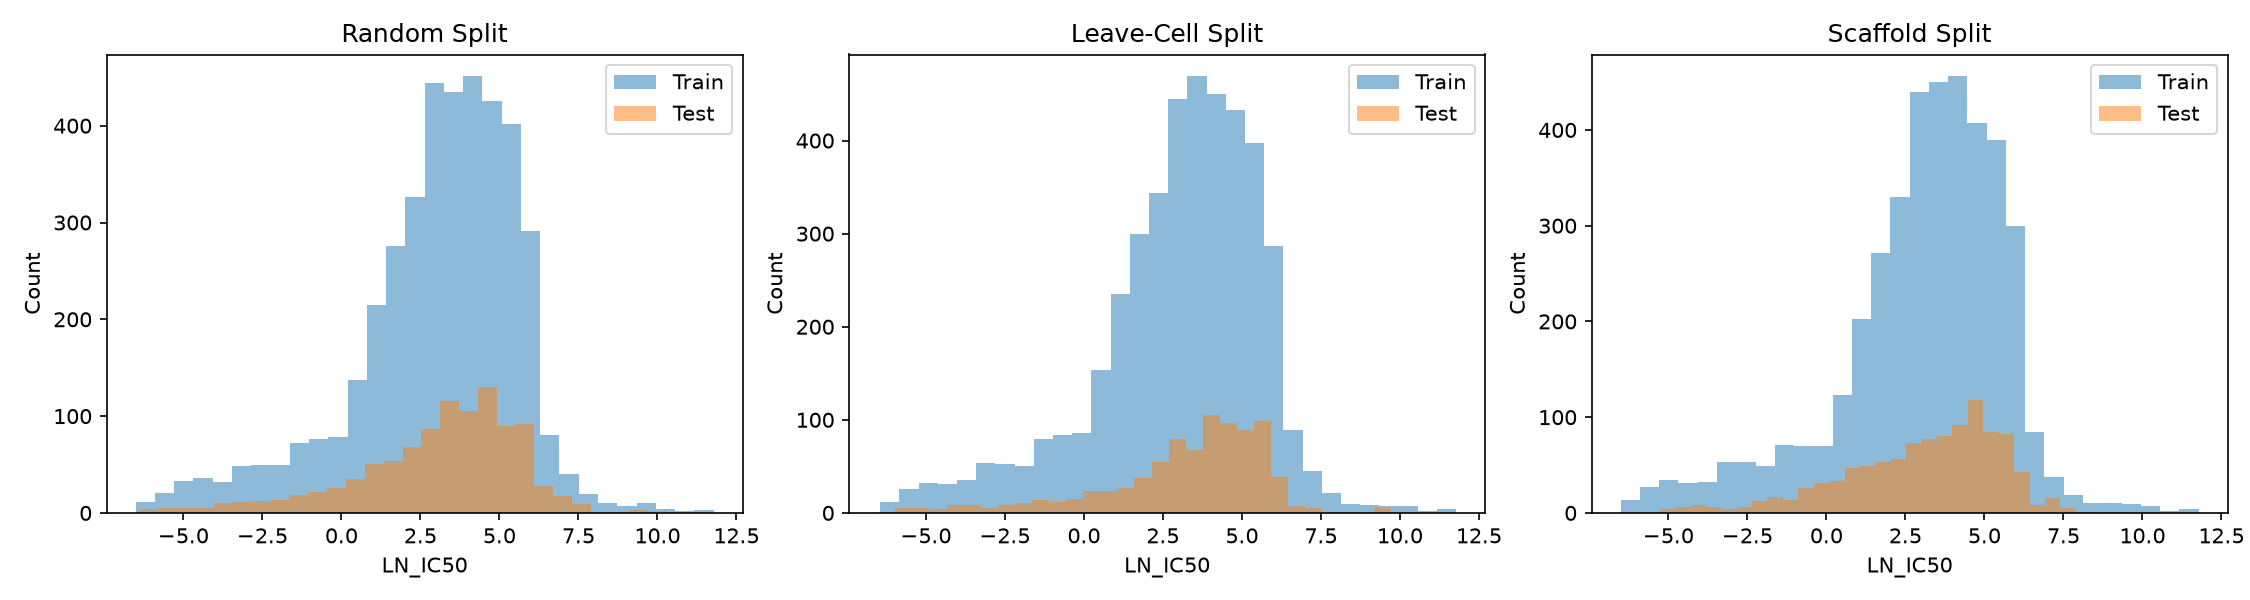
\includegraphics[width=0.76\linewidth]{figures/three_split.png}
  \vspace{-6pt}
  \caption{Train and test $\text{LN\_IC50}$ label distributions across the Random, Leave-Cell-Out, and Bemis--Murcko Scaffold splits ($5,107$ total pairs across $24$ GBM cell lines and $243$ drugs).}
  \label{fig:three_split}
\end{figure}

\paragraph{Qualitative biological and pharmacological examples.}
The dataset reflects key clinical contrasts in GBM: cell line \texttt{U-87 MG} (\texttt{ACH-000075}) has silenced/low \texttt{MGMT} expression ($\text{MGMT\_Expr} = 0.420$) with a \texttt{PTEN} mutation, whereas \texttt{T98G} (\texttt{ACH-000571}) has high \texttt{MGMT} expression ($\text{MGMT\_Expr} = 5.840$) and dual \texttt{PTEN}/\texttt{TP53} mutations, conferring TMZ resistance. Across drugs, standard oral alkylator Temozolomide (scaffold \texttt{O=c1ncc2ncn([H])c2n1}) has a high mean in-vitro $\text{LN\_IC50}$ of $+6.45$, Irinotecan has $+2.76$, Carmustine (BCNU) has $+5.63$, and microtubule inhibitor Docetaxel has $-4.12$.

\section{Approach}
\label{sec:approach}

\subsection{Leakage-free omics standardization and automated pipeline auditing}
Applying standardization or PCA across all cell lines before splitting leaks test-set gene covariance into training features. In \path{src/standardization.py} (\texttt{fit\_transform\_cell\_pca\_features}), we fit all transformations strictly on unique training cell lines $\mathcal{C}_{\text{train}}$:
(1) a per-gene Z-score \texttt{StandardScaler} ($\boldsymbol{\mu}_{\text{train}}, \boldsymbol{\sigma}_{\text{train}}$) is fitted only on $\mathbf{X}_{\text{expr}}^{\text{train}} \in \mathbb{R}^{|\mathcal{C}_{\text{train}}| \times 19,138}$;
(2) PCA is fitted on the scaled training cells with $K = \min(32, |\mathcal{C}_{\text{train}}| - 1)$ components, yielding $K = 23$ on Random/Scaffold ($24$ training cells) and $K = 19$ on Leave-Cell-Out ($20$ training cells), and test cells $\mathcal{C}_{\text{test}}$ are projected onto the frozen axes;
(3) concatenating the $K$ PCA coordinates, $20$ binary hotspot mutations, and training-median-imputed \texttt{MGMT\_Expr} yields $\mathbf{x}_c \in \mathbb{R}^{d_{\text{cell}}}$ with $d_{\text{cell}} = 44$ (Random/Scaffold) or $d_{\text{cell}} = 40$ (Leave-Cell-Out).
After splitting, \path{src/pipeline_audit.py} (\texttt{run\_full\_pipeline\_audit}) programmatically asserts zero pair overlap, zero cell overlap on \texttt{leave\_cell}, zero scaffold overlap on \texttt{scaffold}, removal of raw \texttt{EXPR\_*} columns, and zero NaNs.

\subsection{Closed-form statistical and chemical similarity baselines}
To separate marginal main effects from learned drug--cell interactions, \path{src/baselines.py} defines three closed-form statistical baselines from training means ($\bar{y}_{d,\cdot}$ for drug $d$, $\bar{y}_{\cdot,c}$ for cell line $c$, and global mean $\bar{y}_{\text{train}}$):
\begin{equation}
  \hat{y}^{\text{cell}}_{d,c} = \bar{y}_{\cdot,c}, \qquad
  \hat{y}^{\text{drug}}_{d,c} = \bar{y}_{d,\cdot}, \qquad
  \hat{y}^{\text{add}}_{d,c} = \bar{y}_{d,\cdot} + \bar{y}_{\cdot,c} - \bar{y}_{\text{train}}.
  \label{eq:additive}
\end{equation}
On Leave-Cell-Out, $\bar{y}_{\cdot,c}$ has $0\%$ test coverage; on Scaffold, $\bar{y}_{d,\cdot}$ has $0\%$ test coverage. For unseen drugs $d'$ on the Scaffold split, we also evaluate a \textbf{Nearest-Drug Morgan FP Baseline} (\texttt{evaluate\_nearest\_drug\_scaffold\_baseline}), which predicts $\hat{y}^{\text{NN}}_{d',c} = \bar{y}_{d^*(d'),\cdot}$ using the training drug $d^*(d') = \arg\max_{d \in \mathcal{D}_{\text{train}}} \frac{\mathbf{f}_{d'}^\top \mathbf{f}_d}{\|\mathbf{f}_{d'}\|_2 \|\mathbf{f}_d\|_2}$ with highest Morgan fingerprint cosine similarity.

\subsection{Two-Tower multimodal neural network architecture and training}
Our primary neural architecture is the Two-Tower Multi-Layer Perceptron (\texttt{BaselineMLP} in \path{src/mlp_model.py}), which implements \textbf{Joint (Intermediate) Fusion---Type I} (\emph{MD6329 Lecture 08, Slide 32}~\cite{huang2020fusion}) by encoding drug Morgan fingerprints $\mathbf{f}_d \in \mathbb{R}^{2048}$ and cell multi-omics vectors $\mathbf{x}_c \in \mathbb{R}^{d_{\text{cell}}}$ into $\mathbb{R}^{256}$ intermediate representations before joint concatenation:
\begin{align}
  \mathbf{h}_{\text{drug}} &= \mathbf{W}_{d,2}\,\text{Dropout}_{0.3}\!\left(\text{ReLU}(\mathbf{W}_{d,1}\mathbf{f}_d + \mathbf{b}_{d,1})\right) + \mathbf{b}_{d,2} \in \mathbb{R}^{256}, \quad (2048 \to 512 \to 256), \\
  \mathbf{h}_{\text{cell}} &= \mathbf{W}_{c,2}\,\text{Dropout}_{0.3}\!\left(\text{ReLU}(\mathbf{W}_{c,1}\mathbf{x}_c + \mathbf{b}_{c,1})\right) + \mathbf{b}_{c,2} \in \mathbb{R}^{256}, \quad (d_{\text{cell}} \to 128 \to 256), \\
  \hat{z}_{d,c} &= \mathbf{w}_{\text{out}}^\top\,\text{Dropout}_{0.3}\!\left(\text{ReLU}\!\left(\mathbf{W}_{\text{fuse}}[\mathbf{h}_{\text{drug}} \,\|\, \mathbf{h}_{\text{cell}}] + \mathbf{b}_{\text{fuse}}\right)\right) + b_{\text{out}} \in \mathbb{R}, \quad (512 \to 128 \to 1).
\end{align}
We also implement an exploratory Graph Isomorphism Network (\texttt{GNNDrugMLP}) using two \texttt{GINConv} layers ($16 \to 128 \to 256$) with global mean pooling over SMILES molecular graphs (\path{src/dataset.py}).

\paragraph{Training procedure and Software 3.0 engineering contributions.}
Target $\text{LN\_IC50}$ values are Z-score standardized using training statistics ($\mu_y, \sigma_y$) and trained under MSE loss using Adam ($\eta = 10^{-4}$, weight decay $\lambda = 10^{-4}$, batch size $64$, dropout $0.30$ in \path{src/mlp_training.py}) across $5$ seeds ($\text{seed} \in \{0,\dots,4\}$) for up to $100$ epochs with early stopping patience $15$ on validation RMSE. Predictions are unstandardized via $\hat{y}_{d,c} = \sigma_y \hat{z}_{d,c} + \mu_y$. Using DeepSeek (for modular system architecture design) and Gemini (for code implementation), we refactored our exploratory notebooks into a two-layer package of $15$ atomic modules and $5$ workflow orchestrators (\texttt{src/}). Human verification resolved two AI-generated bugs during refactoring: dynamically inferring $d_{\text{cell}} \in \{40, 44\}$ rather than hardcoding $44$, and adding cell-line stratification in \texttt{partition\_train\_validation}.

\section{Experiments}
\label{sec:experiments}

\subsection{Evaluation metrics and RQ1: Shortcut decomposition on the Random split}
We report four metric groups: (1) \textbf{Global Spearman ($r_s$) and RMSE} across all test pairs ($5$-seed mean $\pm$ SD); (2) \textbf{Within-Cell Spearman} across drugs per cell line ($\ge 10$ drugs); (3) \textbf{Median Within-Drug Spearman} across cell lines per drug ($\ge 10$ cells on Scaffold, $\ge 3$ on Random/Leave-Cell); and (4) \textbf{Prediction variance shrinkage} $\sigma(\hat{y})/\sigma(y)$, mean signed bias, and large-error fraction $|\hat{y} - y| > 2.0\,\ln\mu\text{M}$ (\path{src/uncertainty.py}).

\begin{table}[t]
  \caption{Benchmark comparison of statistical baselines and Two-Tower \texttt{BaselineMLP} ($5$ random seeds, mean $\pm$ SD) across the three evaluation regimes ($5,107$ GBM pairs). ``N/A'' indicates $0\%$ test coverage due to unseen cell lines or unseen drug scaffolds.}
  \label{tab:main_benchmark}
  \centering
  \small
  \resizebox{\textwidth}{!}{%
  \begin{tabular}{lcccccccc}
    \toprule
    Split Regime & Cell-Only $r_s$ & Drug-Only $r_s$ & Additive $r_s$ & Nearest-FP $r_s$ & \texttt{BaselineMLP} Global $r_s$ & \texttt{BaselineMLP} RMSE & Within-Cell MLP $r_s$ & Within-Drug Med.\ $r_s$ \\
    \midrule
    Random (In-Dist.)     & $0.2107$ & $0.8349$ & $\mathbf{0.8752}$ & ---      & $0.8744 \pm 0.0051$ & $\mathbf{1.0346 \pm 0.0211}$ & $0.8541 \pm 0.0576$ & $0.500$ \\
    Leave-Cell-Out (All 5)& N/A      & $0.8362$ & N/A               & ---      & $0.6947 \pm 0.2979$ & $1.3970 \pm 0.6115$          & $\mathbf{0.8460 \pm 0.0608}$ & $0.500$ \\
    Leave-Cell-Out (4 Stable)$^*$ & N/A & $0.8362$ & N/A            & ---      & $\mathbf{0.8436 \pm 0.0034}$ & $\mathbf{1.0912 \pm 0.0085}$ & $\mathbf{0.8460 \pm 0.0608}$ & $0.500$ \\
    Scaffold (Chem.\ OOD) & $0.2494$ & N/A      & N/A               & $0.1445$ & $\mathbf{0.2905 \pm 0.0045}$ & $2.1951 \pm 0.0081$          & $0.1735 \pm 0.0813$ & $\mathbf{0.530}$ \\
    \bottomrule
  \end{tabular}%
  }
  \vspace{1pt}
  \footnotesize{$^*$On Leave-Cell-Out, seeds $0, 1, 3, 4$ converge stably ($r_s \in [0.8388, 0.8476]$), whereas seed $2$ early-stops at epoch $21$ ($r_s = 0.0989$, RMSE $= 2.6199$). Within-Cell Drug-Only achieves $0.8554 \pm 0.0598$ on Random and $0.8449 \pm 0.0602$ on Leave-Cell-Out.}
\end{table}

\begin{figure}[t]
  \centering
  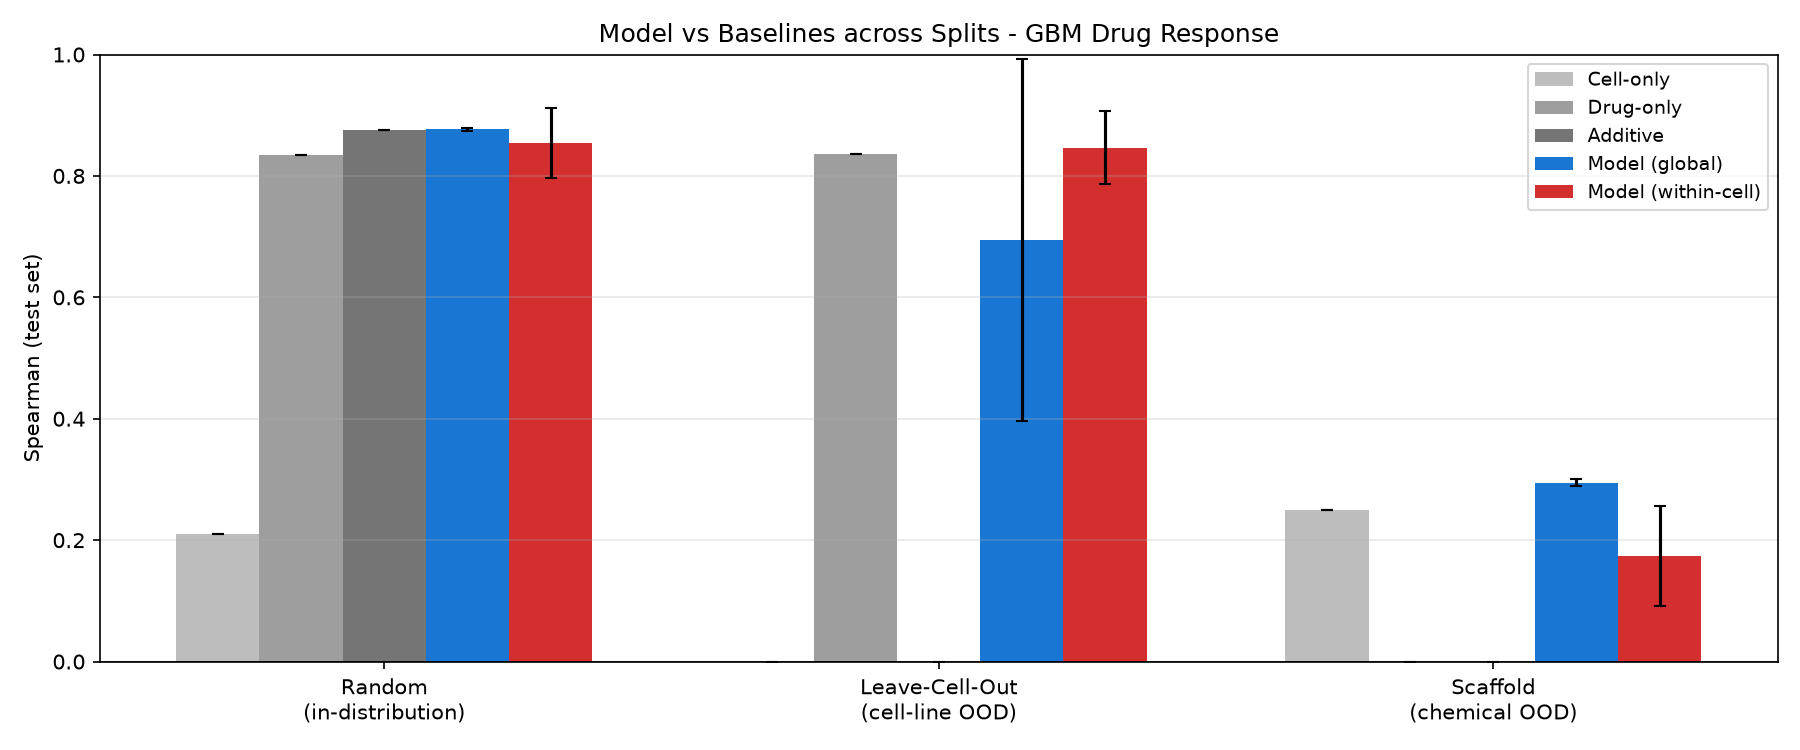
\includegraphics[width=0.75\linewidth]{figures/OOD_three_split_comparison.png}
  \vspace{-6pt}
  \caption{Comparison of statistical baselines (\texttt{Cell-only}, \texttt{Drug-only}, \texttt{Additive}) and \texttt{BaselineMLP} (global and within-cell Spearman) across Random, Leave-Cell-Out, and Scaffold splits. Error bars denote $\pm 1$ standard deviation across $5$ random seeds.}
  \label{fig:three_split_comparison}
\end{figure}

Table~\ref{tab:main_benchmark} and Figure~\ref{fig:three_split_comparison} answer \textbf{RQ1}. On the Random split ($1,022$ test pairs), \texttt{BaselineMLP} achieves a global Spearman of $0.8744 \pm 0.0051$ (RMSE $1.0346 \pm 0.0211$). However, predicting only the marginal cell-line mean (\texttt{Cell-Only}) yields $0.2107$, whereas predicting only the marginal training drug mean (\texttt{Drug-Only}, ignoring all patient omics) yields $0.8349$---explaining $95.5\%$ of the deep network's rank correlation. Adding marginal drug and cell means without interaction (\texttt{Additive} baseline, Eq.~\ref{eq:additive}) achieves $0.8752$, matching \texttt{BaselineMLP} ($0.8744$, net interaction gain $\Delta r_s = -0.0008 \approx 0$). Within individual cell lines, ranking drugs by their training mean (\texttt{Within-Cell Drug-Only} $= 0.8554 \pm 0.0598$) also matches \texttt{BaselineMLP} ($0.8541 \pm 0.0576$, $\Delta r_s = -0.0013$). Thus, high random-split correlation is overwhelmingly driven by memorizing per-drug average toxicity.

\subsection{RQ2: Biological OOD vs.\ Chemical OOD and variance shrinkage}

\paragraph{Biological OOD (Leave-Cell-Out) and multi-seed stability.}
On Leave-Cell-Out ($4$ unseen GBM cell lines, $858$ pairs), \texttt{Drug-Only} achieves $0.8362$ globally and $0.8449 \pm 0.0602$ within-cell because drug potency ordering is conserved across GBM cell lines. Four of five neural network seeds ($\text{seed} \in \{0, 1, 3, 4\}$) converge stably to $r_s = 0.8436 \pm 0.0034$ (RMSE $1.0912 \pm 0.0085$), whereas $\text{seed}=2$ early-stops at epoch $21$ with $r_s = 0.0989$ (RMSE $2.6199$), lowering the $5$-seed mean to $0.6947 \pm 0.2979$ (Table~\ref{tab:main_benchmark}). With only $20$ training cell lines, validation loss on a small subset can plateau prematurely if initial cell-tower weights are poorly aligned, demonstrating why multi-seed auditing (\path{src/uncertainty.py}) is essential.

\begin{table}[t]
  \caption{Prediction variance shrinkage ($\sigma(\hat{y})/\sigma(y)$), signed bias ($\text{mean}(\hat{y}-y)$), large-error rate ($|\hat{y}-y| > 2.0\,\ln\mu\text{M}$), and per-drug median metrics across splits.}
  \label{tab:shrinkage}
  \centering
  \small
  \resizebox{\textwidth}{!}{%
  \begin{tabular}{lccccccc}
    \toprule
    Split Regime & Pred SD $\sigma(\hat{y})$ & True SD $\sigma(y)$ & Shrinkage $\sigma(\hat{y})/\sigma(y)$ & Mean Bias & Frac.\ $|e| > 2.0$ & Per-Drug Med.\ RMSE & Within-Drug Med.\ $r_s$ \\
    \midrule
    Random (In-Dist.)     & $2.267$ & $2.631$ & $0.862$ & $-0.055$ & $6.0\%$  & $0.893$ & $0.500$ \\
    Leave-Cell-Out (OOD)  & $2.209$ & $2.592$ & $0.852$ & $-0.147$ & $7.0\%$  & $0.887$ & $0.500$ \\
    Scaffold (Chem.\ OOD) & $1.630$ & $2.459$ & $\mathbf{0.663}$ & $-0.316$ & $\mathbf{36.8\%}$ & $\mathbf{1.644}$ & $\mathbf{0.530}$ \\
    \bottomrule
  \end{tabular}%
  }
\end{table}

\begin{figure}[t]
  \centering
  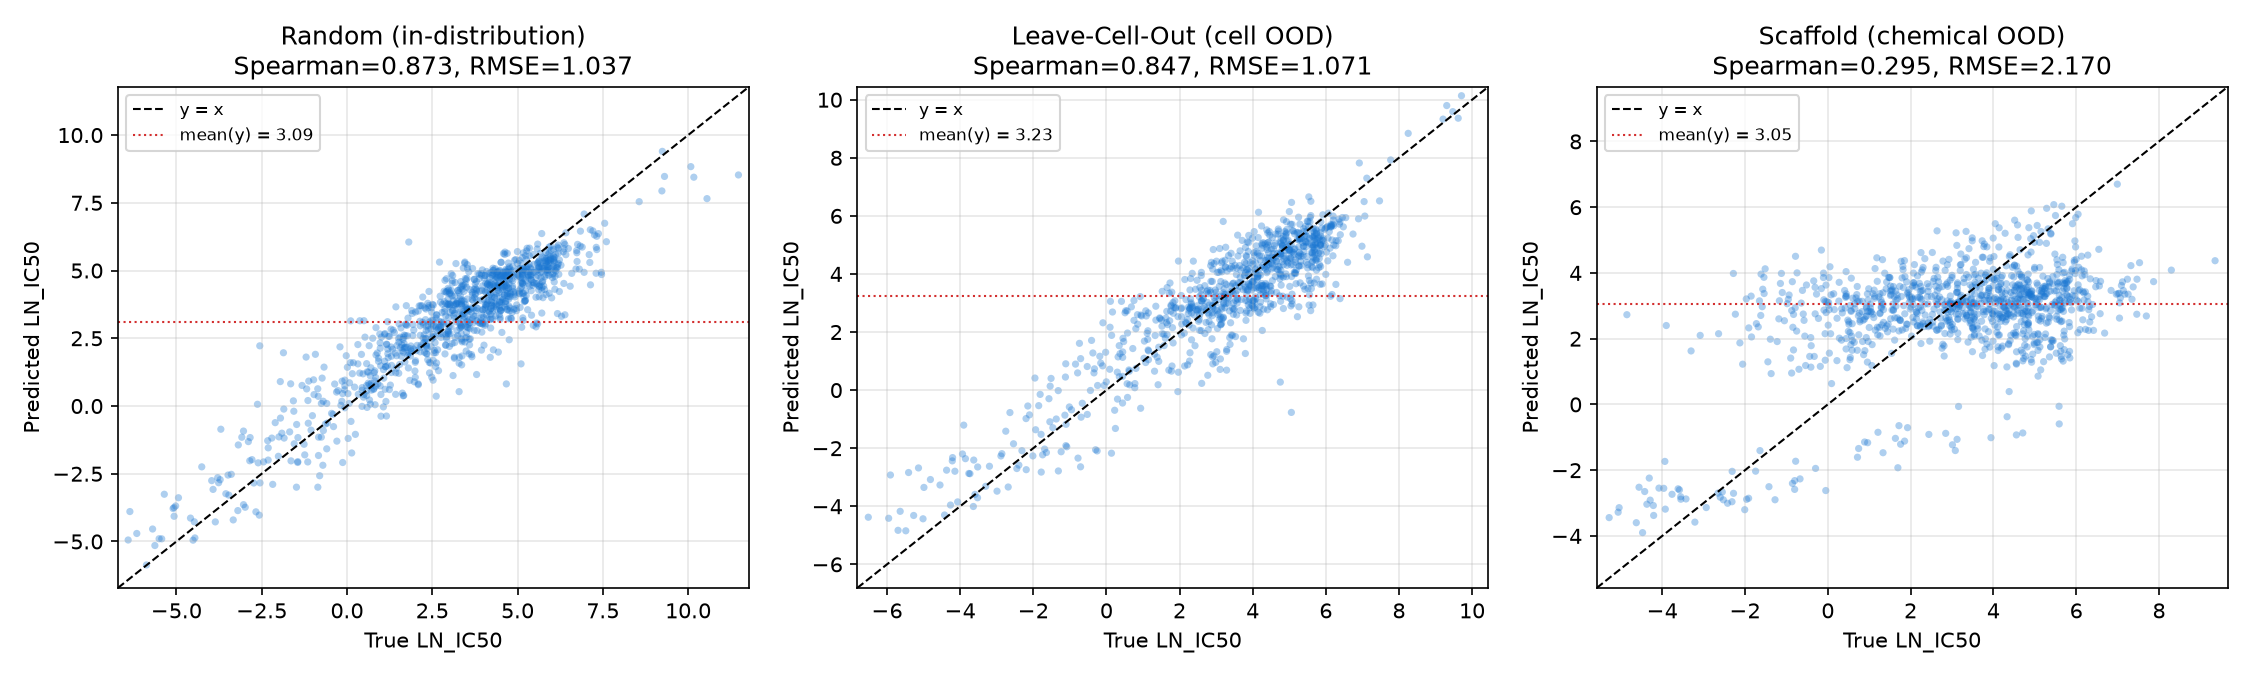
\includegraphics[width=0.80\linewidth]{figures/OOD_scatter_three_splits.png}
  \vspace{-6pt}
  \caption{Predicted vs.\ true $\text{LN\_IC50}$ scatter plots across Random (left), Leave-Cell-Out (middle), and Bemis--Murcko Scaffold (right) test sets. On the Scaffold split, unseen chemical structures cause predictions to compress horizontally toward the global training mean ($\bar{y} \approx 2.85$--$3.05$, red dotted line), reducing $\sigma(\hat{y})/\sigma(y)$ from $0.862$ to $0.663$.}
  \label{fig:scatter_three_splits}
\end{figure}

\paragraph{Chemical OOD (Scaffold split) and variance shrinkage.}
On the Scaffold split ($47$ unseen drugs, $1,051$ pairs), drug-identity lookup is impossible (\texttt{Drug-Only} coverage $= 0\%$). Global Spearman drops from $0.8744$ to $0.2905 \pm 0.0045$, Within-Cell Spearman drops to $0.1735 \pm 0.0813$, and RMSE doubles from $1.0346$ to $2.1951 \pm 0.0081$ (though \texttt{BaselineMLP} still doubles the correlation of \texttt{Nearest-Drug Morgan FP} at $0.1445$). As shown in Table~\ref{tab:shrinkage} and Figure~\ref{fig:scatter_three_splits}, unfamiliar Morgan fingerprints cause drug-tower outputs to regress toward the global training mean under MSE loss: the shrinkage ratio $\sigma(\hat{y})/\sigma(y)$ contracts from $0.862$ (Random) and $0.852$ (Leave-Cell-Out) to $0.663$ (Scaffold), and the fraction of test predictions with $|\hat{y} - y| > 2.0\,\ln\mu\text{M}$ jumps from $6.0\%$ to $36.8\%$.

\subsection{RQ3: Decoupling between global collapse and within-drug patient ranking}
Comparing global pooled correlation against within-drug correlation across cell lines reveals our central technical finding (Table~\ref{tab:shrinkage} and Figure~\ref{fig:decoupling_and_novelty}, left): while global Spearman drops from $0.8744$ to $0.2905$ on the Scaffold split, the \textbf{median within-drug Spearman across the $24$ GBM cell lines remains $0.530$} (compared to $0.500$ on Random and $0.500$ on Leave-Cell-Out).

\begin{figure}[t]
  \centering
  \begin{minipage}[t]{0.44\linewidth}
    \centering
    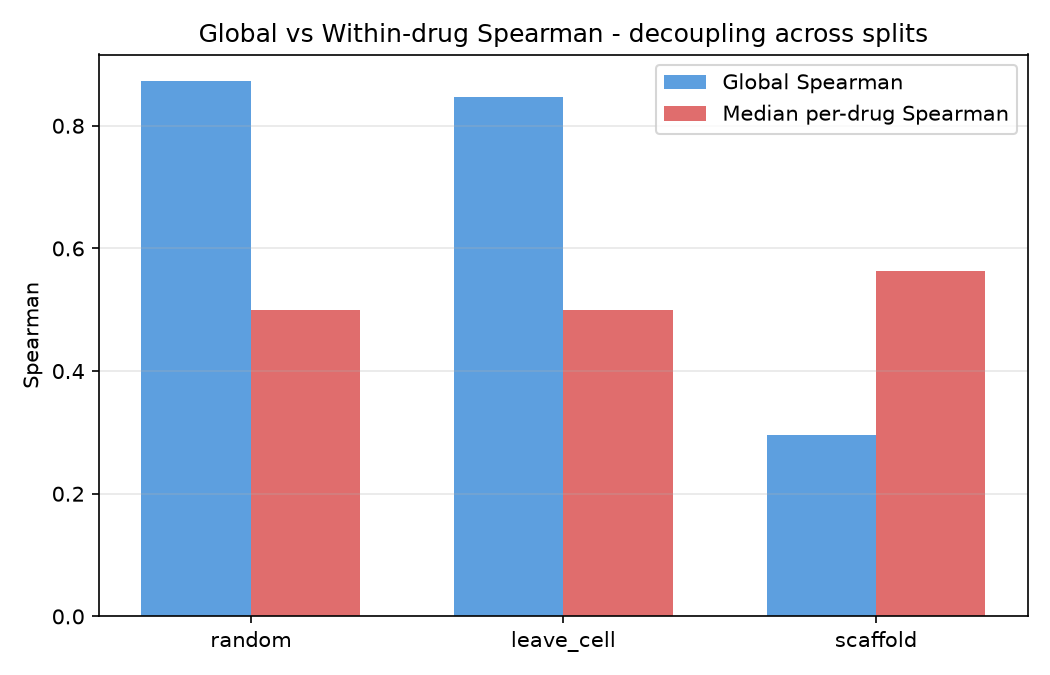
\includegraphics[width=\linewidth]{figures/OOD_global_vs_within_drug_spearman.png}
  \end{minipage}\hfill
  \begin{minipage}[t]{0.44\linewidth}
    \centering
    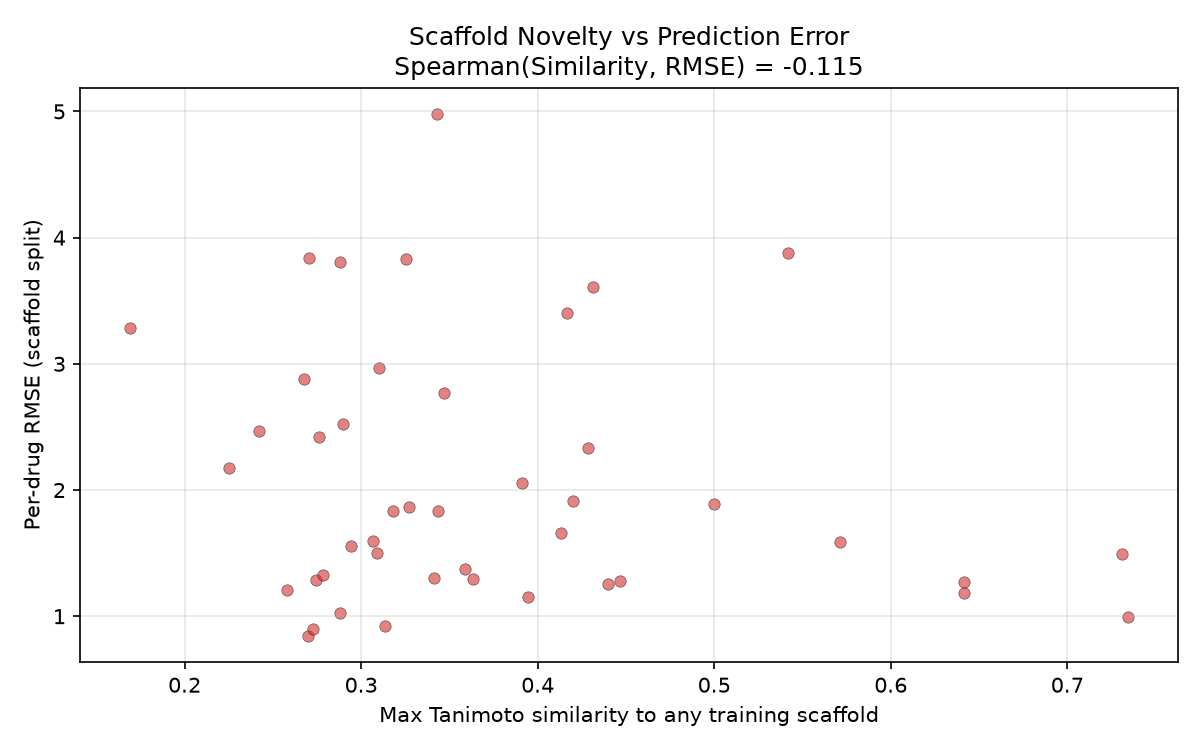
\includegraphics[width=\linewidth]{figures/OOD_scaffold_novelty_vs_error.png}
  \end{minipage}
  \vspace{-6pt}
  \caption{\emph{Left:} Decoupling between global pooled Spearman (blue) and median within-drug Spearman across GBM cell lines (red) across splits. \emph{Right:} Per-drug RMSE on the Scaffold split vs.\ maximum Tanimoto similarity to any training scaffold ($r_s = -0.115$).}
  \label{fig:decoupling_and_novelty}
\end{figure}

Mathematically, for a fixed unseen drug $d_0$, the drug embedding $\mathbf{h}_{\text{drug}}(d_0)$ is constant across all $24$ GBM cell lines. Misestimating the baseline potency of $d_0$ adds a constant offset $\Delta_{d_0}$ to every cell line's prediction for that compound. Because rank ordering within drug $d_0$ is invariant to a constant shift $\Delta_{d_0}$, the cell tower---which was trained on all $24$ cell lines---still ranks relative patient susceptibility from multi-omics profiles ($r_s = 0.530$). When all $47$ unseen drugs are pooled together, however, the uncalibrated offsets $\{\Delta_d\}$ corrupt cross-drug rankings and collapse global Spearman ($0.2905$).

\subsection{Clinical GBM drug audit, scaffold novelty, and Software 3.0 testing}

\begin{table}[t]
  \caption{Audit of four clinical GBM chemotherapeutics across splits (\texttt{inspect\_key\_gbm\_drugs}) and scaffold novelty RMSE bins (\texttt{analyze\_scaffold\_novelty\_vs\_error}).}
  \label{tab:clinical_and_novelty}
  \centering
  \small
  \resizebox{\textwidth}{!}{%
  \begin{tabular}{llccccclccc}
    \toprule
    \multicolumn{6}{c}{\textbf{(a) Clinical GBM Drugs Audit Across Splits}} & & \multicolumn{4}{c}{\textbf{(b) Scaffold Split Tanimoto Similarity vs.\ RMSE}} \\
    \cmidrule(r){1-6} \cmidrule(l){8-11}
    Drug Name & Split & $n$ & True Mean & Pred Mean & Bias / RMSE & & Max Train Tanimoto & Drugs & Mean RMSE & Median RMSE \\
    \midrule
    Temozolomide & Random   & $3$  & $+6.45$ & $+6.17$ & $-0.28$ / $0.50$ & & $< 0.30$ (High novelty)    & $15$ & $2.112$ & $\mathbf{2.161}$ \\
    Temozolomide & Scaffold & $22$ & $+6.45$ & $+3.32$ & $\mathbf{-3.13}$ / $\mathbf{3.23}$ & & $0.30\text{--}0.50$ (Moderate) & $23$ & $2.120$ & $1.871$ \\
    Irinotecan   & Random   & $4$  & $+2.76$ & $+2.69$ & $-0.07$ / $0.72$ & & $0.50\text{--}0.70$ (Near-analog)& $4$  & $2.020$ & $1.463$ \\
    Irinotecan   & Scaffold & $21$ & $+2.76$ & $-1.01$ & $\mathbf{-3.78}$ / $\mathbf{3.92}$ & & $> 0.70$ (Close scaffold)  & $2$  & $1.253$ & $\mathbf{1.253}$ \\
    Carmustine   & Leave-Cell& $1$ & $+5.63$ & $+5.15$ & $-0.49$ / $0.87$ & & \multicolumn{4}{l}{\footnotesize{Continuous Spearman$(S_{\max}, \text{RMSE}) = -0.115$}} \\
    Etoposide    & Random   & $4$  & $+2.24$ & $+1.88$ & $-0.36$ / $0.90$ & & \multicolumn{4}{l}{\footnotesize{($72\%$ higher median RMSE for $<0.30$ vs.\ $>0.70$)}} \\
    \bottomrule
  \end{tabular}%
  }
\end{table}

Table~\ref{tab:clinical_and_novelty}a shows the impact of variance shrinkage on clinical GBM drugs. For Temozolomide (TMZ), Random-split predictions are well-calibrated (true $+6.45$, pred $+6.17$, RMSE $0.50$), but on the Scaffold split ($S_{\max} = 0.284$), predictions shrink toward the global mean ($\sim 2.85$) to $+3.32$, causing a $-3.13$ log-unit bias (RMSE $3.23$). Likewise, Irinotecan ($S_{\max} = 0.241$) shifts from RMSE $0.72$ on Random to $-3.78$ log bias (RMSE $3.92$) on Scaffold. Across all held-out drugs (Table~\ref{tab:clinical_and_novelty}b and Figure~\ref{fig:decoupling_and_novelty}, right), highly novel scaffolds ($S_{\max} < 0.30$) suffer a $72\%$ higher median RMSE ($2.161$) than close analogs ($S_{\max} > 0.70$, median RMSE $1.253$). Finally, Gemini assisted in building our $58$-test unit suite (\texttt{tests/}), automated GitHub Actions CI (\path{.github/workflows/ci.yml}), single-file project showcase (\path{docs/index.html}), and interactive \texttt{LecTrace}\footnote{LecTrace interactive execution-explanation framework by Mr.\ Adesanmi Dayo Praisegod: \url{https://pypi.org/project/lectrace/}.} script (\path{Lectrace/01_gbm_ood_presentation.py}), which traces (1) train-only standardization, (2) a forward pass showing a $+1.258\,\ln\mu\text{M}$ resistance shift between \texttt{MGMT}-low \texttt{U-87 MG} and \texttt{MGMT}-high \texttt{T98G} on TMZ, (3) additive shortcut decomposition, and (4) chemical OOD shrinkage.

\section{Conclusion}
\label{sec:conclusion}

We presented a leakage-free multimodal benchmark auditing shortcut learning and out-of-distribution generalization across $5,107$ GDSC2 and DepMap Glioblastoma drug--cell pairs ($24$ GBM cell lines and $243$ small-molecule drugs). Our study yields three main findings for precision oncology machine learning:
\begin{enumerate}
  \setlength{\itemsep}{1.5pt}\setlength{\parskip}{0pt}\setlength{\topsep}{2pt}
  \item \textbf{In-distribution correlation is dominated by drug-mean memorization:} On the Random split, a closed-form zero-interaction \texttt{Additive} baseline ($r_s = 0.8752$) matches our Two-Tower \texttt{BaselineMLP} ($0.8744 \pm 0.0051$), with $95.5\%$ of explainable rank correlation driven by per-drug average toxicity (\texttt{Drug-Only} $r_s = 0.8349$). Preclinical drug response benchmarks should report additive baselines alongside neural network metrics to rule out shortcut learning.
  \item \textbf{Chemical OOD shift induces severe prediction variance shrinkage:} While biological OOD (Leave-Cell-Out) preserves high correlation across stable seeds ($0.8436$), holding out unseen Bemis--Murcko chemical scaffolds reduces global Spearman to $0.2905 \pm 0.0045$ and compresses prediction standard deviation ($\sigma(\hat{y})/\sigma(y) = 0.663$), causing large systematic potency offsets on clinical GBM agents such as Temozolomide ($-3.13$ log units) and Irinotecan ($-3.78$ log units).
  \item \textbf{Relative patient stratification survives chemical OOD:} Despite global collapse on unseen scaffolds, median within-drug Spearman across the $24$ GBM cell lines remains $0.530$. Thus, while current multi-omics neural networks must not be used to select uncalibrated clinical dosages for novel compounds, their cell-line encoders retain signal for ranking relative patient susceptibility in biomarker-stratified oncology trials.
\end{enumerate}

\paragraph{Limitations and future work.}
First, GDSC2 assays measure 72-hour in-vitro viability in 2D immortalized cell lines, which do not capture blood--brain barrier permeability, tumor microenvironment interactions, or systemic toxicity in patients. Second, our cohort is limited to $24$ GBM cell lines; expanding to patient-derived glioma stem-like cells (GSCs) will improve statistical power for Leave-Cell-Out evaluation. Future work will investigate pre-trained 3D molecular foundation encoders to mitigate chemical OOD shrinkage and few-shot single-concentration calibration to anchor baseline potency offsets for novel scaffolds.

\subsubsection*{Acknowledgments}
We express our sincere gratitude to our course instructor, Prof.\ Chee Wei Tan, and the series of invited guest lecturers in \emph{MD6329: Deep Learning in Healthcare AI} at Nanyang Technological University for their insightful lectures and guidance on experimental design, out-of-distribution auditing, and responsible healthcare AI evaluation. We thank Mr.\ Adesanmi Dayo Praisegod, creator of the open-source \texttt{LecTrace} project, for providing the interactive execution-explanation presentation framework and lecture demonstration. We also acknowledge open-source data and software contributions from the GDSC~\cite{yang2013gdsc,iorio2016landscape}, DepMap/CCLE~\cite{tsherniak2017depmap,ghandi2019next}, PyTorch~\cite{paszke2019pytorch}, PyTorch Geometric~\cite{fey2019fast}, Scikit-learn~\cite{pedregosa2011scikit}, and RDKit~\cite{landrum2016rdkit} projects. Regarding Generative AI tools, DeepSeek was used to assist with initial ideation, problem formulation, and modular project architecture design, while Gemini was used to assist with code implementation, frontend showcase page design, and report writing/\LaTeX{} typesetting; all experimental hypotheses, baseline derivations, code execution, and scientific interpretations were independently verified by the author.

\section*{References}

\medskip
\small
\renewcommand{\section}[2]{}%

\begin{thebibliography}{27}

\bibitem{stupp2005radiotherapy}
Stupp, R., Mason, W.P., van den Bent, M.J., Weller, M., Fisher, B., Taphoorn, M.J., Belanger, K., Brandes, A.A., Marosi, C., Bogdahn, U., et al.\ (2005)
Radiotherapy plus concomitant and adjuvant temozolomide for glioblastoma.
\emph{New England Journal of Medicine} \textbf{352}(10):987--996.

\bibitem{hegi2005mgmt}
Hegi, M.E., Diserens, A.C., Gorlia, T., Hamou, M.F., de Tribolet, N., Weller, M., Kros, J.M., Hainfellner, J.A., Mason, W., Mariani, L., et al.\ (2005)
\emph{MGMT} gene silencing and benefit from temozolomide in glioblastoma.
\emph{New England Journal of Medicine} \textbf{352}(10):997--1003.

\bibitem{brennan2013somatic}
Brennan, C.W., Verhaak, R.G., McKenna, A., Campos, B., Noushmehr, H., Salama, S.R., Zheng, S., Chakravarty, D., Sanborn, J.Z., Berman, S.H., et al.\ (2013)
The somatic genomic landscape of glioblastoma.
\emph{Cell} \textbf{155}(2):462--477.

\bibitem{yang2013gdsc}
Yang, W., Soares, J., Greninger, P., Edelman, E.J., Lightfoot, H., Forbes, S., Bindal, N., Beare, D., Smith, J.A., Thompson, I.R., et al.\ (2013)
Genomics of Drug Sensitivity in Cancer (GDSC): a resource for therapeutic biomarker discovery in cancer cells.
\emph{Nucleic Acids Research} \textbf{41}(D1):D955--D961.

\bibitem{iorio2016landscape}
Iorio, F., Knijnenburg, T.A., Vis, D.J., Bignell, G.R., Menden, M.P., Schubert, M., Aben, N., Gon{\c{c}}alves, E., Barthorpe, S., Lightfoot, H., et al.\ (2016)
A landscape of pharmacogenomic interactions in cancer.
\emph{Cell} \textbf{166}(3):740--754.

\bibitem{barretina2012ccle}
Barretina, J., Caponigro, G., Stransky, N., Venkatesan, K., Margolin, A.A., Kim, S., Wilson, C.J., Leh{\'a}r, J., Kryukov, G.V., Sonkin, D., et al.\ (2012)
The Cancer Cell Line Encyclopedia enables predictive modelling of anticancer drug sensitivity.
\emph{Nature} \textbf{483}(7391):603--607.

\bibitem{tsherniak2017depmap}
Tsherniak, A., Vazquez, F., Montgomery, P.G., Weir, B.A., Kryukov, G., Cowley, G.S., Gill, S., Harrington, W.F., Pantel, S., Krill-Burger, J.M., et al.\ (2017)
Defining a cancer dependency map.
\emph{Cell} \textbf{170}(3):564--576.

\bibitem{ghandi2019next}
Ghandi, M., Huang, F.W., Jan{\'e}-Valbuena, J., Kryukov, G.V., Lo, C.C., McDonald, E.R., Barretina, J., Gelfand, E.T., Bielski, C.M., Li, H., et al.\ (2019)
Next-generation characterization of the Cancer Cell Line Encyclopedia.
\emph{Nature} \textbf{569}(7757):503--508.

\bibitem{costello2014community}
Costello, J.C., Heiser, L.M., Georgii, E., G{\"o}nen, M., Menden, M.P., Wang, N.J., Bansal, M., Ammad-ud-din, M., Hintsanen, P., Khan, S.A., et al.\ (2014)
A community effort to assess and improve drug sensitivity prediction algorithms.
\emph{Nature Biotechnology} \textbf{32}(12):1202--1212.

\bibitem{chang2018cdrscan}
Chang, Y., Park, H., Yang, H.J., Lee, S., Lee, K.Y., Kim, T.S., Jung, J., \& Shin, J.M.\ (2018)
Cancer Drug Response Profile scan (CDRscan): a deep learning model that predicts drug effectiveness from cancer genomic signature.
\emph{Scientific Reports} \textbf{8}(1):8857.

\bibitem{liu2020deepcdr}
Liu, Q., Hu, Z., Jiang, R., \& Zhou, M.\ (2020)
DeepCDR: a hybrid graph convolutional network for predicting cancer drug response.
\emph{Bioinformatics} \textbf{36}(Supplement\_2):i911--i918.

\bibitem{nguyen2021graphdrp}
Nguyen, T., Nguyen, G.T., Nguyen, T., \& Le, D.H.\ (2021)
Graph convolutional networks for drug response prediction.
\emph{IEEE/ACM Transactions on Computational Biology and Bioinformatics} \textbf{19}(1):146--154.

\bibitem{zhu2022tgsa}
Zhu, Y., Ouyang, Z., Chen, W., Feng, R., Chen, D.Z., Cao, J., \& Wu, J.\ (2022)
TGSA: protein--protein association-based twin graph neural networks for drug response prediction with similarity augmentation.
\emph{Bioinformatics} \textbf{38}(2):461--468.

\bibitem{rogers2010ecfp}
Rogers, D.\ \& Hahn, M.\ (2010)
Extended-connectivity fingerprints.
\emph{Journal of Chemical Information and Modeling} \textbf{50}(5):742--754.

\bibitem{bemis1996properties}
Bemis, G.W.\ \& Murcko, M.A.\ (1996)
The properties of known drugs. 1. Molecular frameworks.
\emph{Journal of Medicinal Chemistry} \textbf{39}(15):2887--2893.

\bibitem{wu2018moleculenet}
Wu, Z., Ramsundar, B., Feinberg, E.N., Gomes, J., Geniesse, C., Pappu, A.S., Leswing, K., \& Pande, V.\ (2018)
MoleculeNet: a benchmark for molecular machine learning.
\emph{Chemical Science} \textbf{9}(2):513--530.

\bibitem{xu2019powerful}
Xu, K., Hu, W., Leskovec, J., \& Jegelka, S.\ (2019)
How powerful are graph neural networks?
In \emph{International Conference on Learning Representations (ICLR)}.

\bibitem{geirhos2020shortcut}
Geirhos, R., Jacobsen, J.H., Michaelis, C., Zemel, R., Brendel, W., Bethge, M., \& Wichmann, F.A.\ (2020)
Shortcut learning in deep neural networks.
\emph{Nature Machine Intelligence} \textbf{2}(11):665--673.

\bibitem{li2021audit}
Li, Y., Umbach, D.M., Krahn, J.M., Shats, I., Li, X., \& Li, L.\ (2021)
Predicting tumor response to drugs based on gene-expression biomarkers of sensitivity learned from cancer cell lines.
\emph{BMC Genomics} \textbf{22}(1):272.

\bibitem{sharifi2021out}
Sharifi-Noghabi, H., Jahangiri-Tazehkand, S., Smirnov, P., Hon, C., Mammoliti, A., Nair, S.K., Mer, A.S., Ester, M., \& Haibe-Kains, B.\ (2021)
Drug sensitivity prediction from cell line-based pharmacogenomics data: guidelines for developing machine learning models.
\emph{Briefings in Bioinformatics} \textbf{22}(6):bbab294.

\bibitem{huang2020fusion}
Huang, S.C., Pareek, A., Seyyedi, S., Banerjee, I., \& Lungren, M.P.\ (2020)
Fusion of medical imaging and electronic health records using deep learning: a systematic review and implementation guidelines.
\emph{NPJ Digital Medicine} \textbf{3}(1):136.

\bibitem{nestor2019feature}
Nestor, B., McDermott, M.B., Boag, W., Berner, G., Naumann, T., Hughes, M.C., Goldenberg, A., \& Ghassemi, M.\ (2019)
Feature robustness in non-stationary health records: caveats to deployable model performance in common clinical machine learning tasks.
In \emph{Machine Learning for Healthcare Conference (MLHC)}, PMLR \textbf{106}:381--405.

\bibitem{mitchell2019model}
Mitchell, M., Wu, S., Zaldivar, A., Barnes, P., Vasserman, L., Hutchinson, B., Spitzer, E., Raji, I.D., \& Gebru, T.\ (2019)
Model cards for model reporting.
In \emph{Proceedings of the Conference on Fairness, Accountability, and Transparency (FAT*)}, pp.\ 220--229.

\bibitem{landrum2016rdkit}
Landrum, G.\ (2016)
RDKit: Open-source cheminformatics software.
\url{https://www.rdkit.org/}.

\bibitem{paszke2019pytorch}
Paszke, A., Gross, S., Massa, F., Lerer, A., Bradbury, J., Chanan, G., Killeen, T., Lin, Z., Gimelshein, N., Antiga, L., et al.\ (2019)
PyTorch: an imperative style, high-performance deep learning library.
In \emph{Advances in Neural Information Processing Systems (NeurIPS)} \textbf{32}, pp.\ 8024--8035.

\bibitem{fey2019fast}
Fey, M.\ \& Lenssen, J.E.\ (2019)
Fast graph representation learning with PyTorch Geometric.
In \emph{ICLR Workshop on Representation Learning on Graphs and Manifolds}.

\bibitem{pedregosa2011scikit}
Pedregosa, F., Varoquaux, G., Gramfort, A., Michel, V., Thirion, B., Grisel, O., Blondel, M., Prettenhofer, P., Weiss, R., Dubourg, V., et al.\ (2011)
Scikit-learn: machine learning in Python.
\emph{Journal of Machine Learning Research} \textbf{12}:2825--2830.

\end{thebibliography}

\end{document}
